\problemname{Bingo}

Ture plays a special kind of bingo that works as follows:
\begin{itemize}
\item He has a square card with $N$x$N$ cells, each containing an integer. The same number may appear in multiple cells.
\item The caller announces one arbitrary integer at a time. If Ture has this number on his card, he may cross it off. If he has the number in multiple cells, he must choose exactly one cell to cross off.
\item When Ture has crossed off a full line of $N$ numbers, either horizontally, vertically, or diagonally (see figure), he has ``bingo'' and wins a trip to BOI (Bingo Olympiad International).
\end{itemize}

Ture does not rely on luck and has cheated to obtain the sequence of numbers that will be called. Write a program that, given Ture's card and the sequence of numbers, computes after how many calls Ture gets bingo if he plays optimally.

\begin{figure}[!h]
\begin{center}
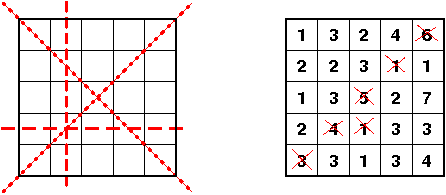
\includegraphics[width=0.6\textwidth]{bingo.png}
\end{center}
\caption{Left: The two diagonal lines (dotted lines) and
  examples of a horizontal and a vertical line (dashed
  lines). Right: A possible way to cross off in the first example.}
\end{figure}



\section*{Input}
The first line contains the integers $N$ and $K$ ($1\leq N \leq 100$, $1 \leq K \leq 10\,000$), the
side length of the card and the number of calls.

Then follow $N$ lines each containing $N$ integers in the interval $1 \ldots 1000$. This is Ture's bingo card.

Finally follows a line with $K$ integers in the same interval, the called numbers in the order they are called.

\section*{Output}
Output an integer: the minimum number of calls needed before Ture gets a full line (horizontally,
vertically, or diagonally). It will never require more than $K$ calls.

\section*{Scoring}
Your solution will be tested on a set of test groups.
To earn points for a group, you must pass all test cases in that group.


\noindent
\begin{tabular}{| l | l | p{12cm} |}
  \hline
  \textbf{Group} & \textbf{Points} & \textbf{Constraints} \\ \hline
  $1$    & $20$       & $K \leq 100$ \\ \hline
  $2$    & $40$       & It is never optimal to try to get bingo along the diagonals. \\ \hline
  $3$    & $40$       & No additional constraints. \\ \hline
\end{tabular}
